\section{関連研究}
\ref{tools} では \ref{sec:intro} 章で述べた,androguard, droidbox についてより詳しく説明する.\ref{researches} で,Android マルウェアを解析,調査した研究を 3 つ紹介する.
\subsection{Android マルウェアを解析するためのツール}
\label{tools}
androgurard \cite{aguard} は Android マルウェアを解析し,クラス同士の関係を表すグラフを作る.このAndroid アプリのクラスの視覚化ツールは Androgexf である.androguard  は Androgexf だけではなく,他にもたくさんのツールを提供しており,その数は全部で 14 にもなる.例えば,その中の 1 つの Androaxml は\ref{sec:andrapp} で説明した,AndroidManifest.xml などのバイナリーの XML を人間が読めるように変換するツールである.Androgexf  に APK ファイルを入力すると,GEXF 形式のファイル (.gexf) として解析結果のグラフを出力する.GEXF ファイルは Gephi というフリーソフトで見ることができる.このグラフはメソッドコールグラフであり,それぞれのノードには,メソッドのタイプ (activity, service, receiver etc) , クラス名,どの権限が使用されているか,その権限のレベル (それぞれの権限には,normal, signature, dangerous などのレベルがある) が記されている.図\ref{androguardgraph} のように,このグラフではどの部分が危険であるかを色を変えて示してあり,どのメソッドが不正な動きをしているかがグラフを見れば簡単にわかる.図\ref{androguardgraph} では,"MONEY\_RISK", "SMS\_RISK" というタグが付けられている.これは,矢印が指されているメソッドのノード,sendSms がバックグラウンドで SMS を送るという危険があることを示している. また,動的にコードをロードしているメソッドも検知することができる.

droidbox \cite{dbox} は Androidのエミュレータ上でマルウェアを実行することで動的に解析する.droidbox  は,端末のネットワークデータのやりとり,ファイルの読み込み・書き込みの命令,ネットワーク,ファイル,または SMS を通じた情報の流出,送信された SMS と電話,開始されたサービス,といった多くの情報を解析する.さらに,解析後は,マルウェアの振る舞いを表す 2 つのグラフも生成する.図\ref{dboxgraph1} , 図\ref{dboxgraph2} はこの 2 つのグラフである.図\ref{dboxgraph1} の縦軸はアプリの活動の種類を表し,横軸は時間である.図\ref{dboxgraph1} の 横軸  30 から 40 にかけて,"net open", "leak" という activity が頻繁に発生している.これはこの間に情報が流出したことを意味する.図\ref{dboxgraph2} は解析した複数のマルウェアの類似性を比較するために用いられる.それぞれの色 (CALL, FILE WRITE, NETLEAK, etc) の領域の割合を比べることで,異なるパッケージのマルウェアがどれほど似た挙動をしているかがわかる.

\begin{figure}[t]
\begin{center}
\graphicspath{{./epsfiles/}}
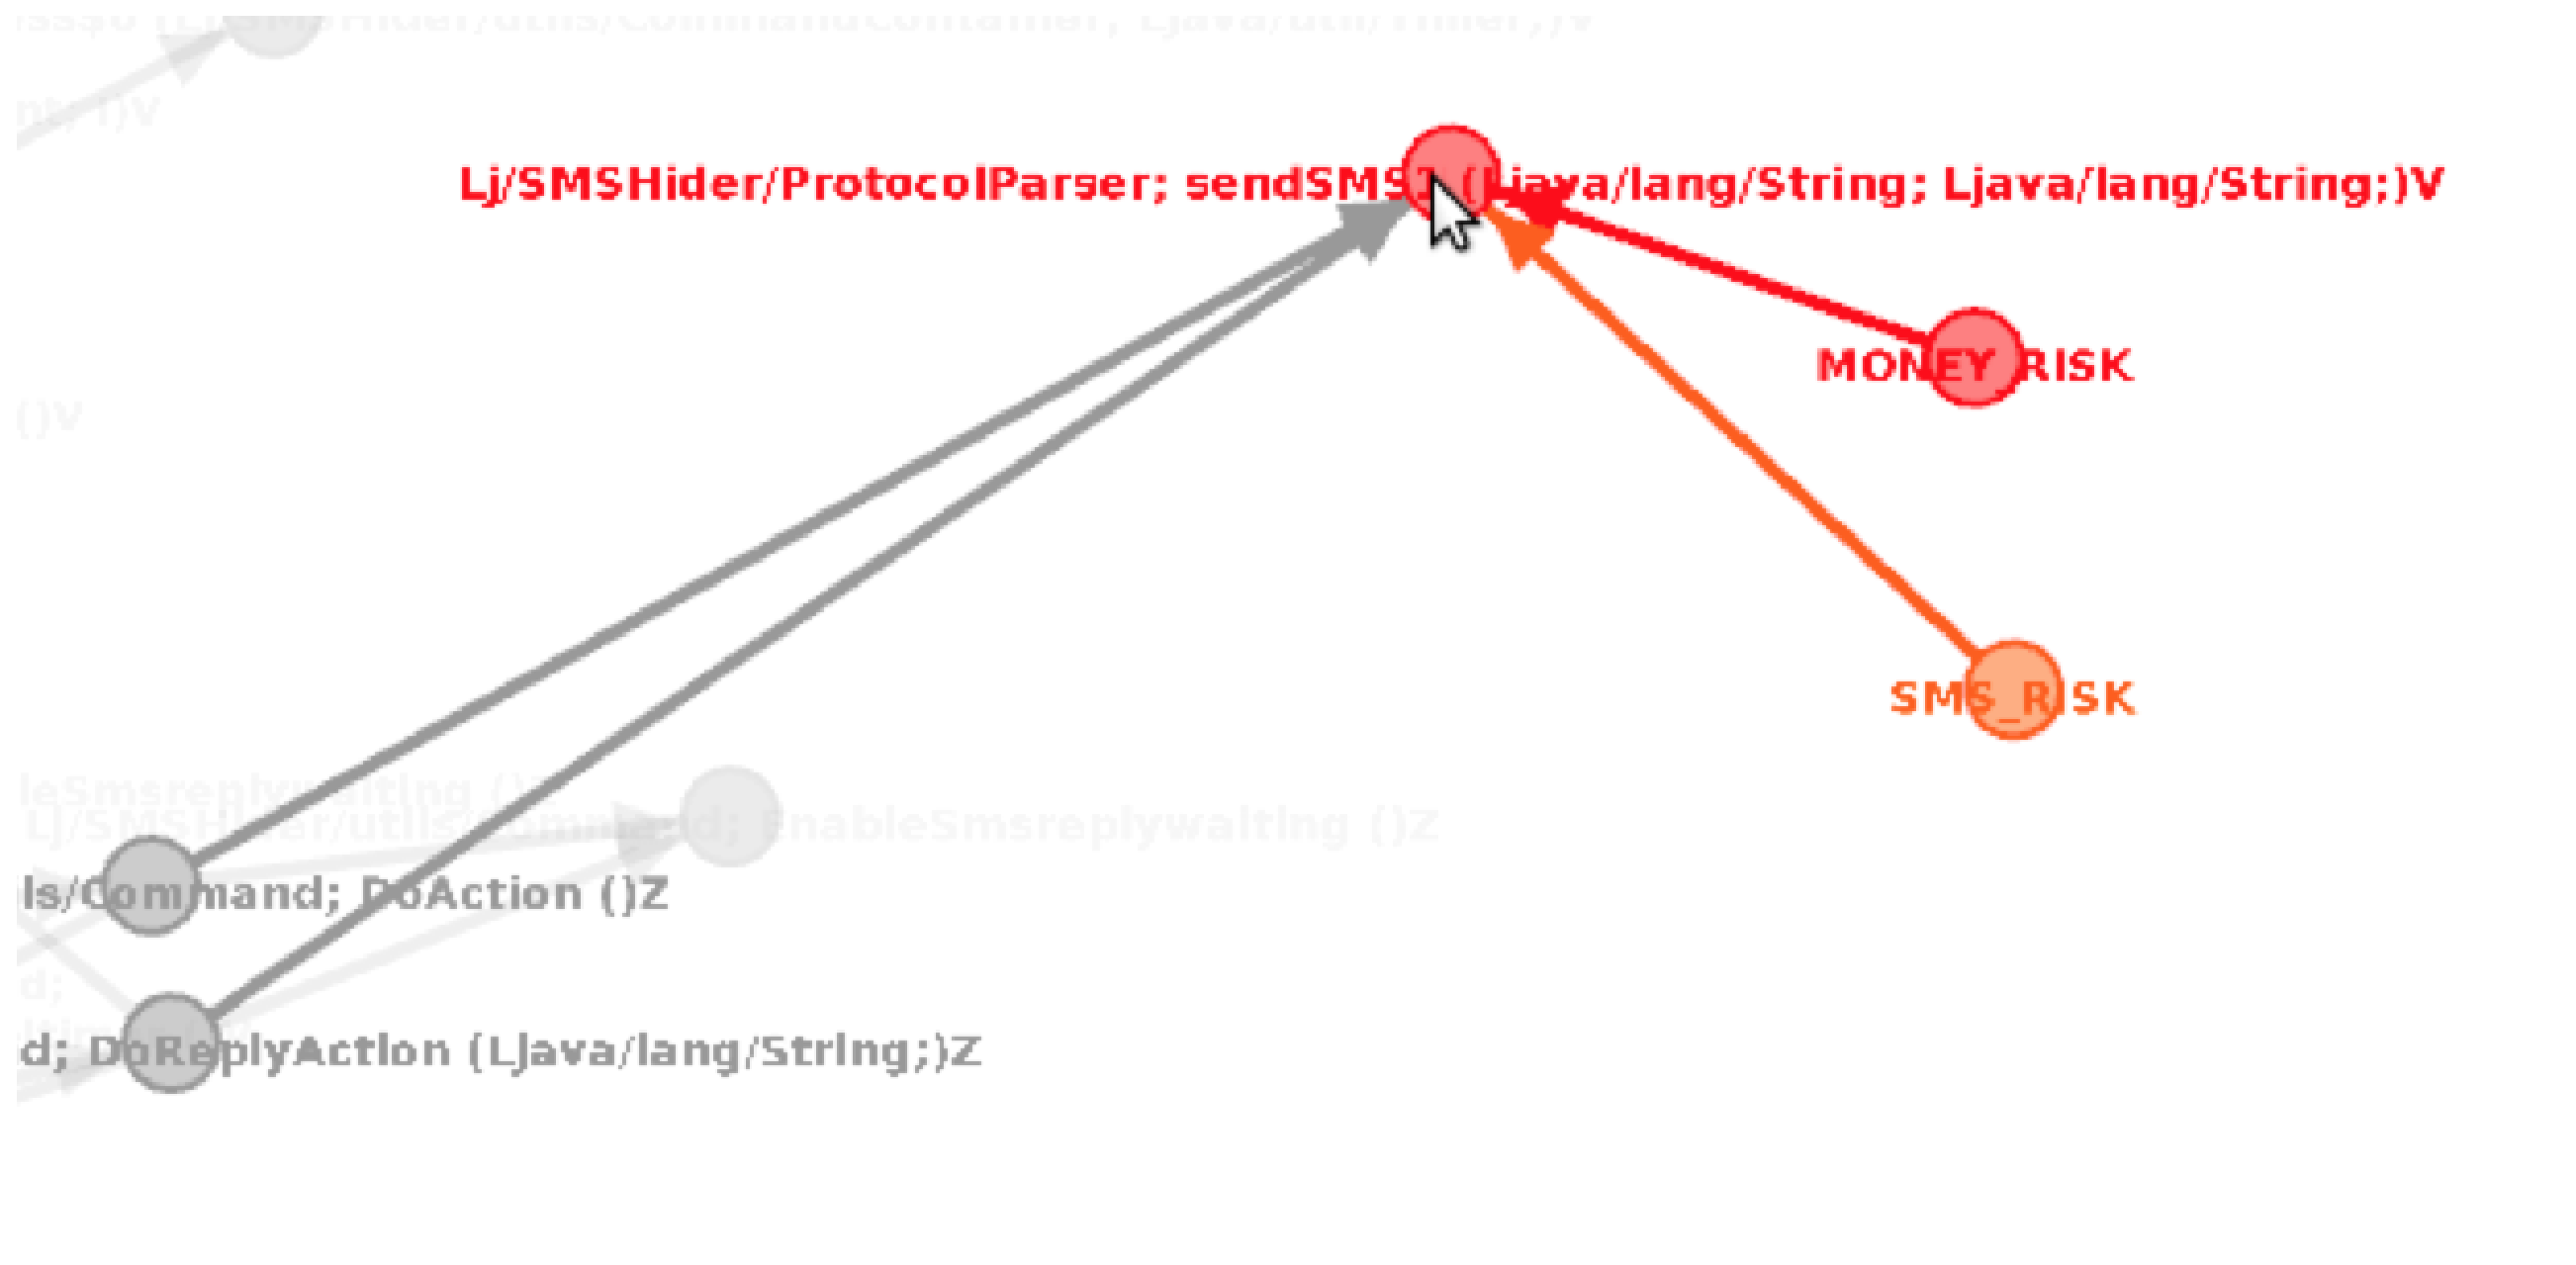
\includegraphics[ scale = 0.3]{androguard.eps}
\end{center}
\caption{androguard が生成するグラフの一部}
\label{androguardgraph}
\end{figure}

\begin{figure}[t]
\begin{center}
\graphicspath{{./epsfiles/}}
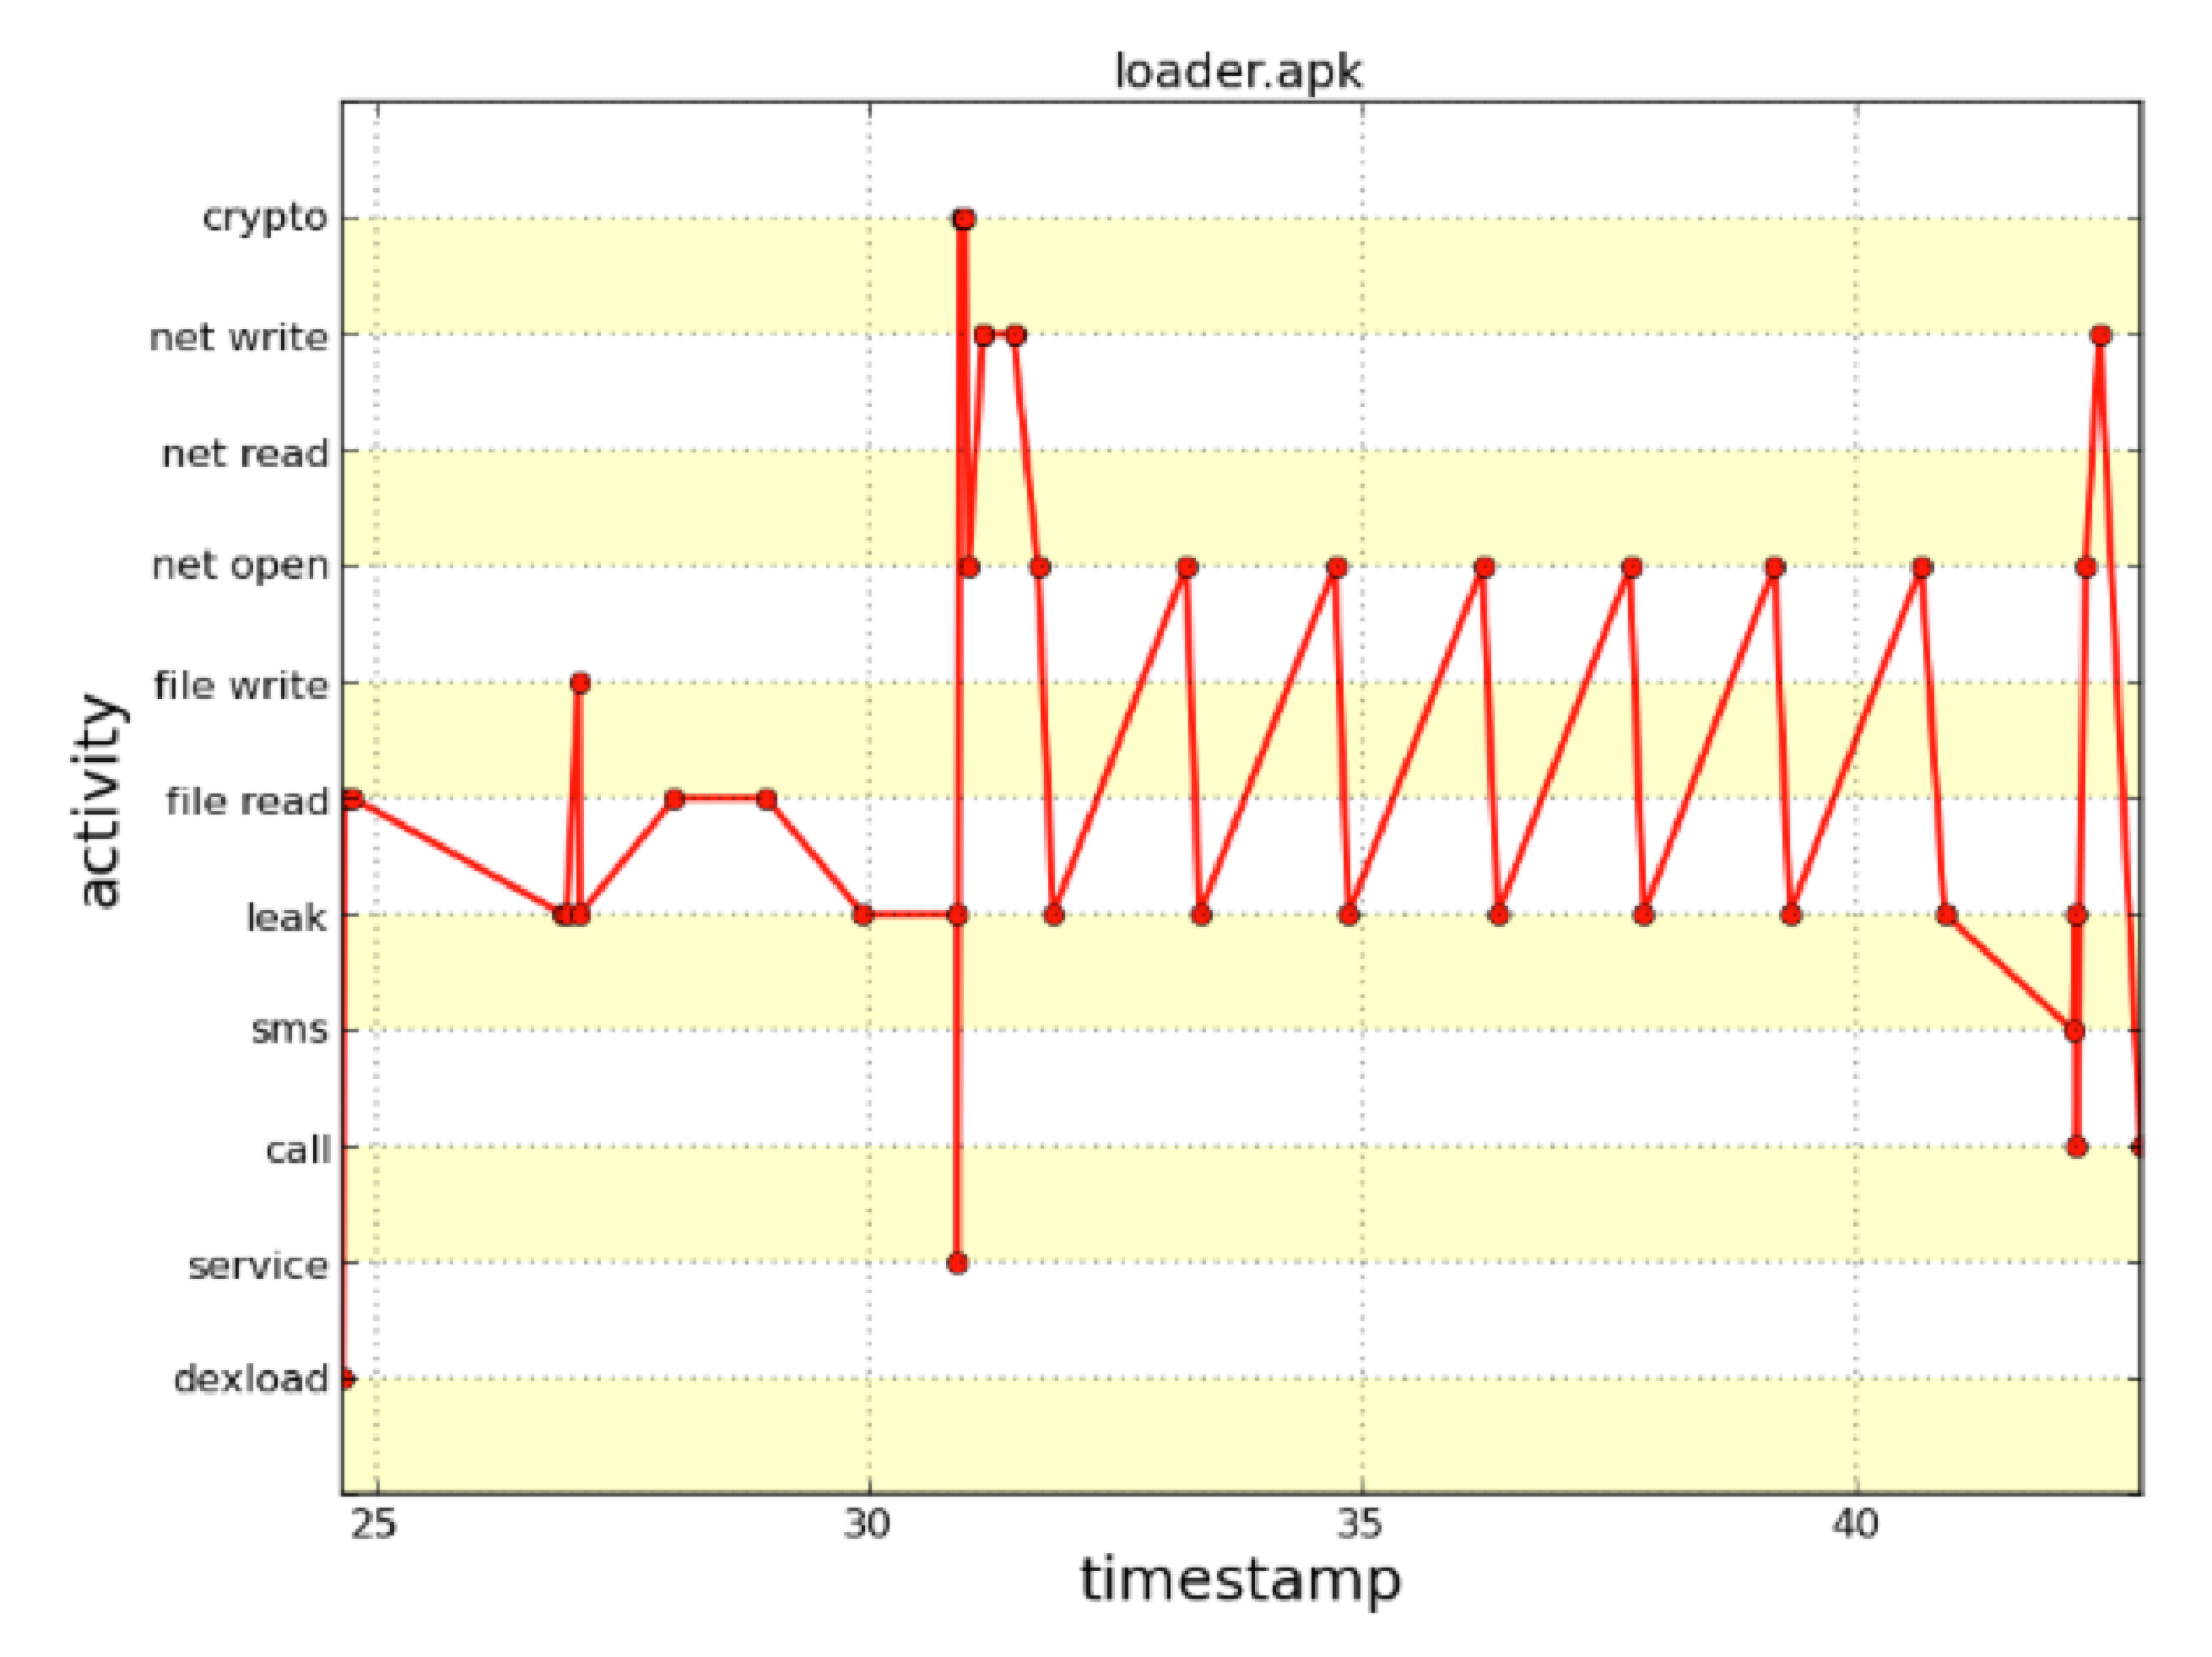
\includegraphics[ scale = 0.2]{droidbox1.eps}
\end{center}
\caption{droidbox の activity の時系列グラフ}
\label{dboxgraph1}
\end{figure}

\begin{figure}[t]
\begin{center}
\graphicspath{{./epsfiles/}}
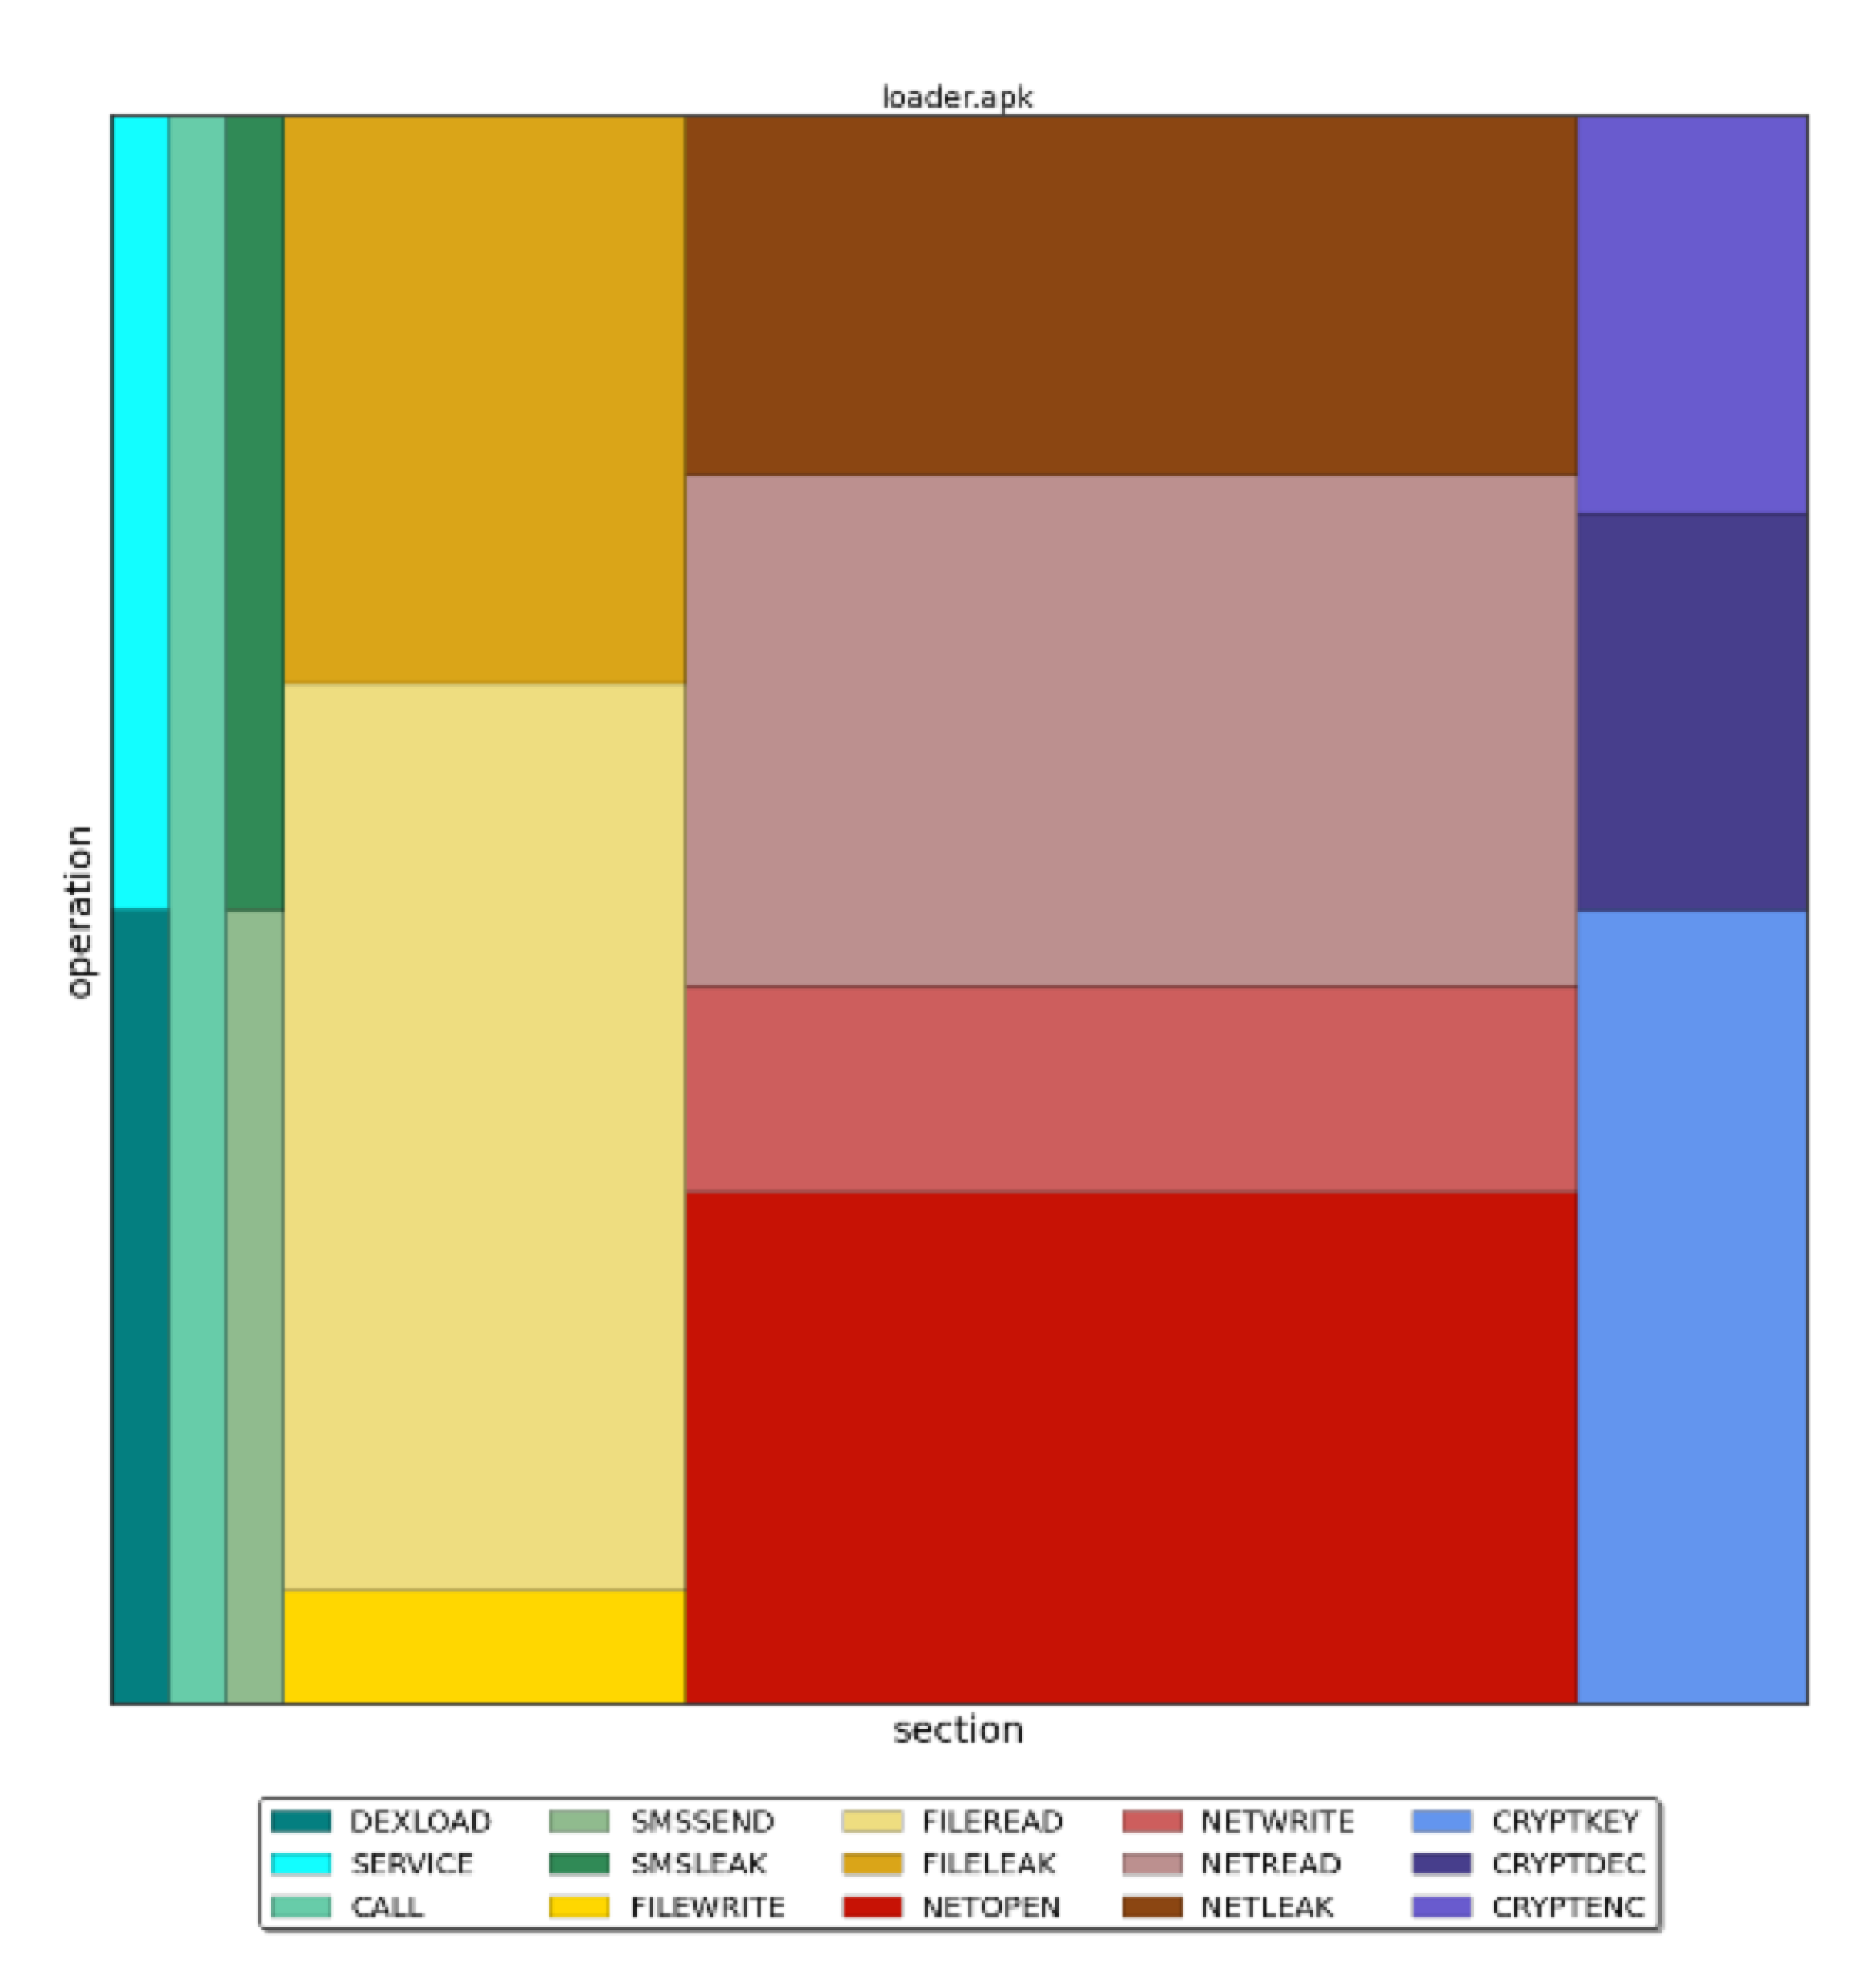
\includegraphics[ scale = 0.2]{droidbox2.eps}
\end{center}
\caption{droidbox の operation - section グラフ}
\label{dboxgraph2}
\end{figure}

\if0
\begin{figure}[t]
	\begin{minipage}{0.5\hsize}
	\begin{center}
		\graphicspath{{./epsfiles/}}
		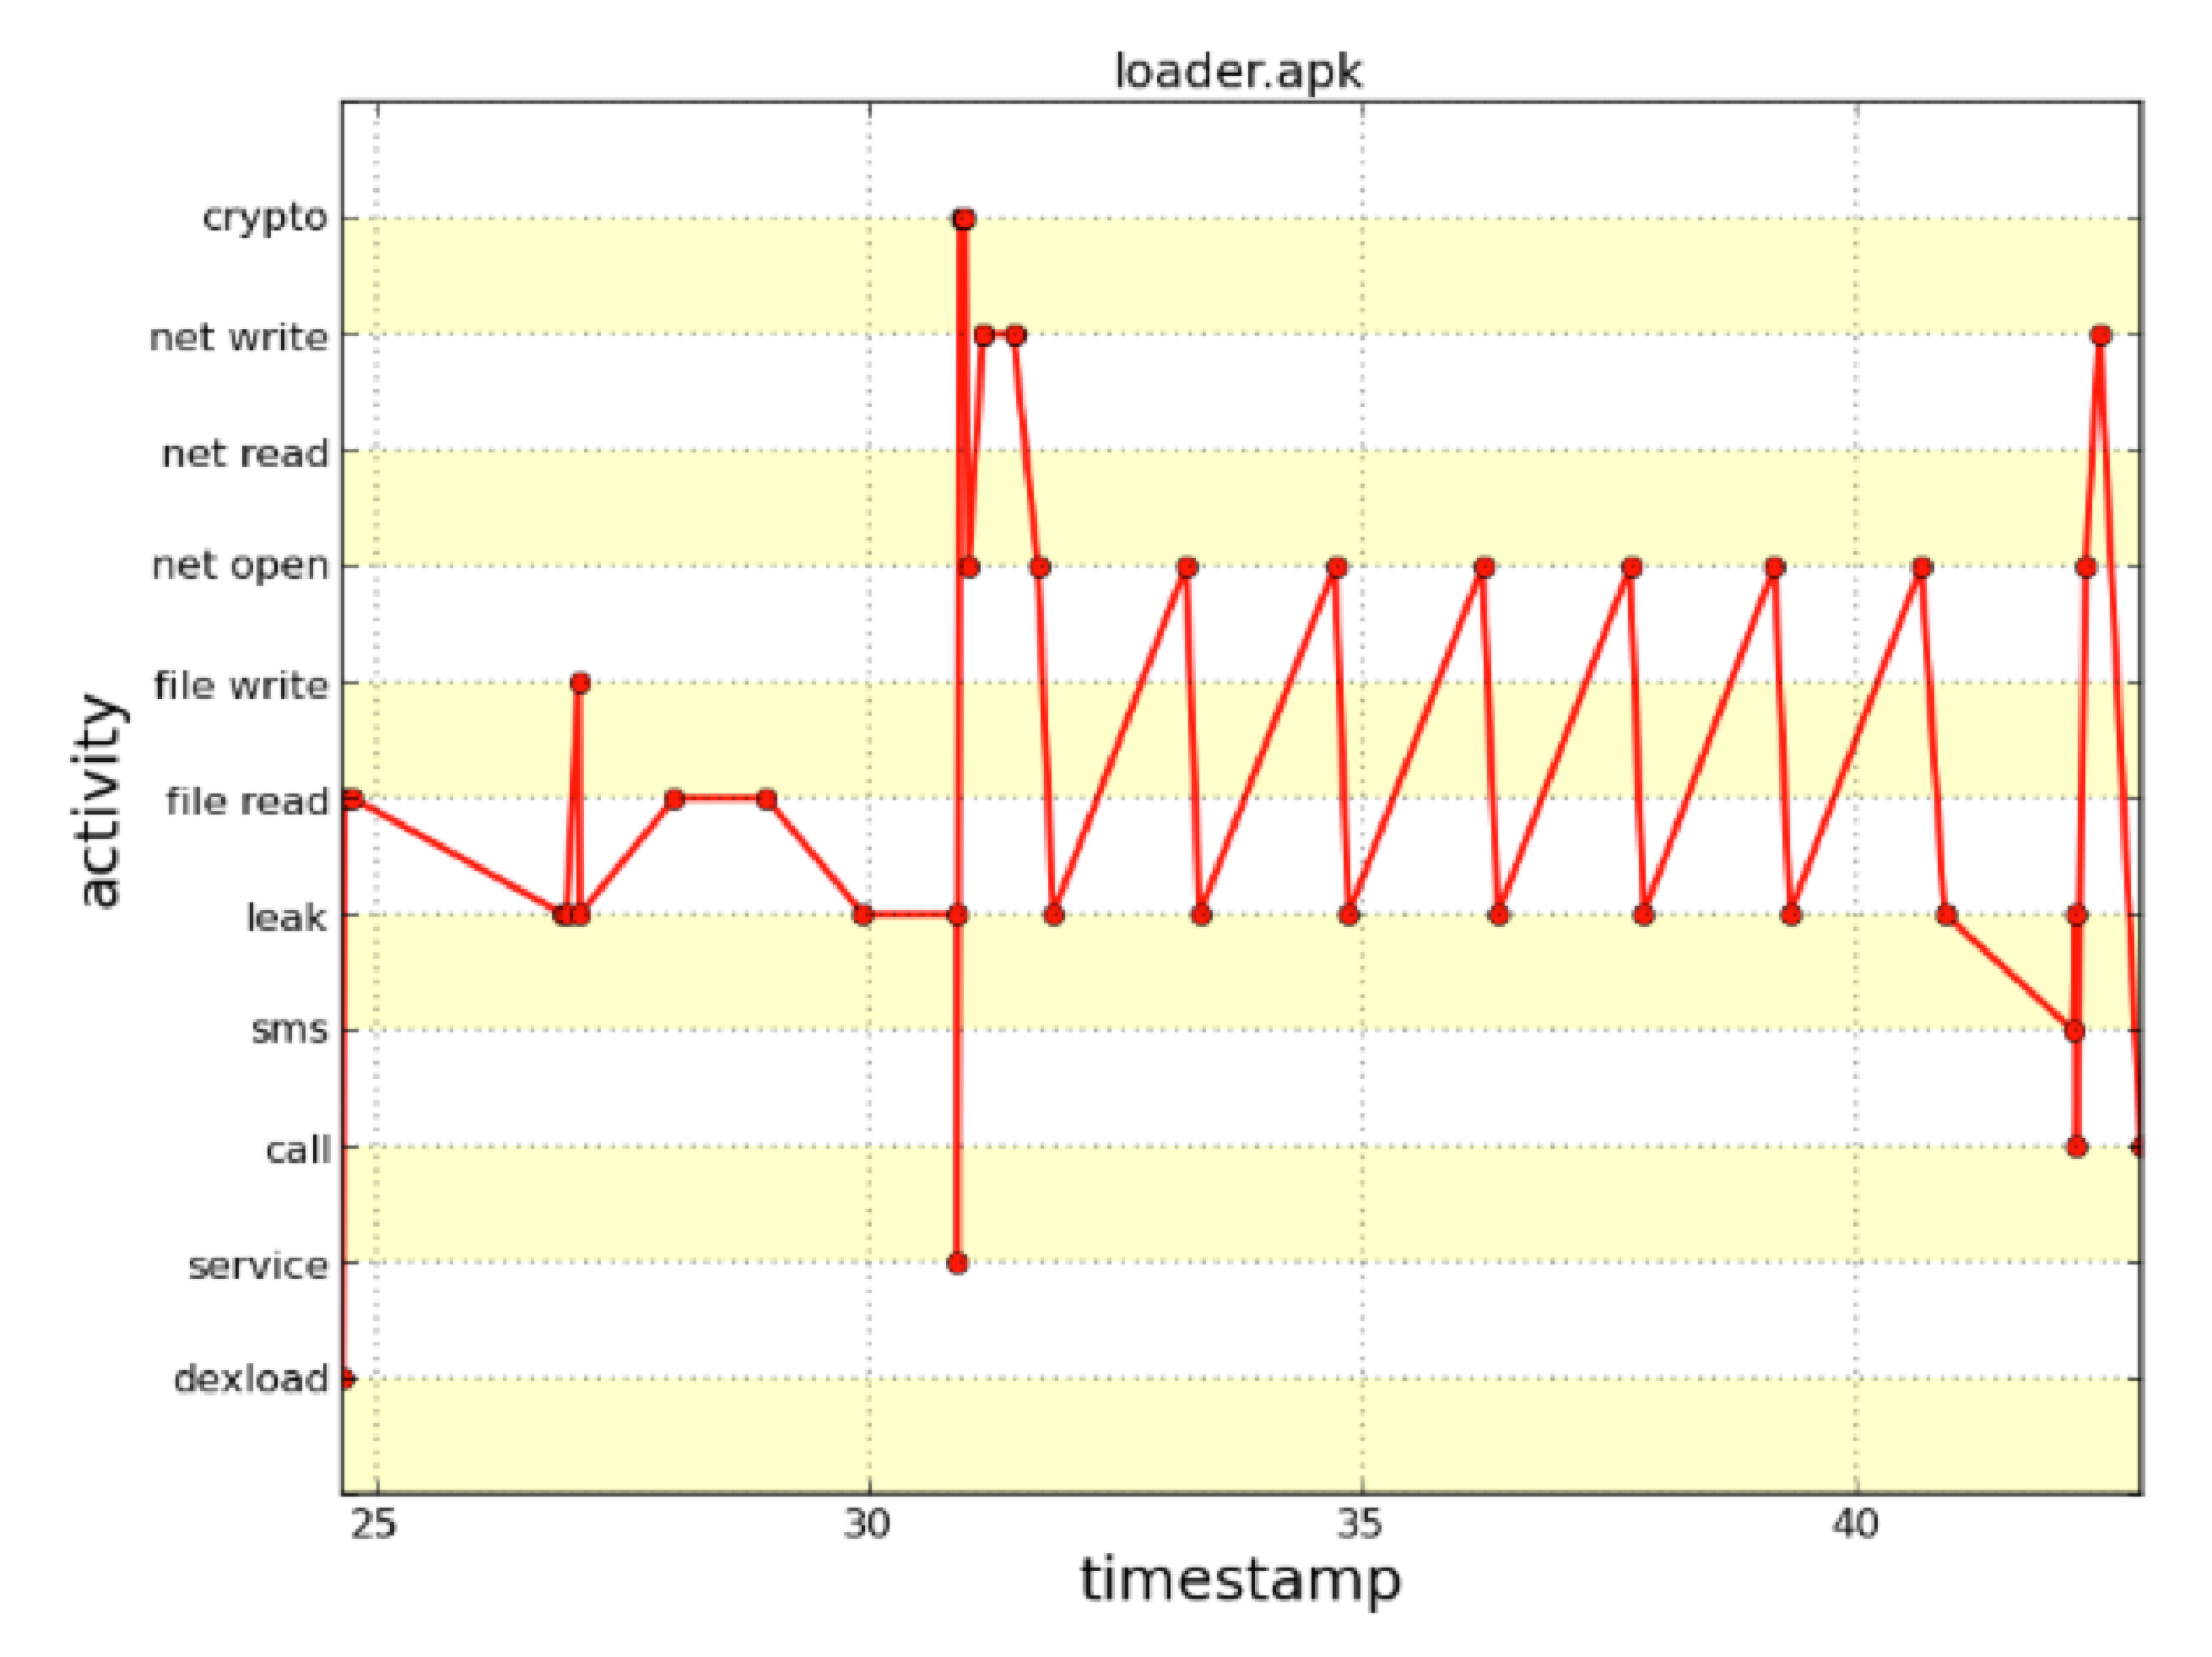
\includegraphics[scale=0.2]{droidbox1.eps}
	\end{center}
	\end{minipage}
	\begin{minipage}{0.5\hsize}
	\begin{center}
		\graphicspath{{./epsfiles/}}	
		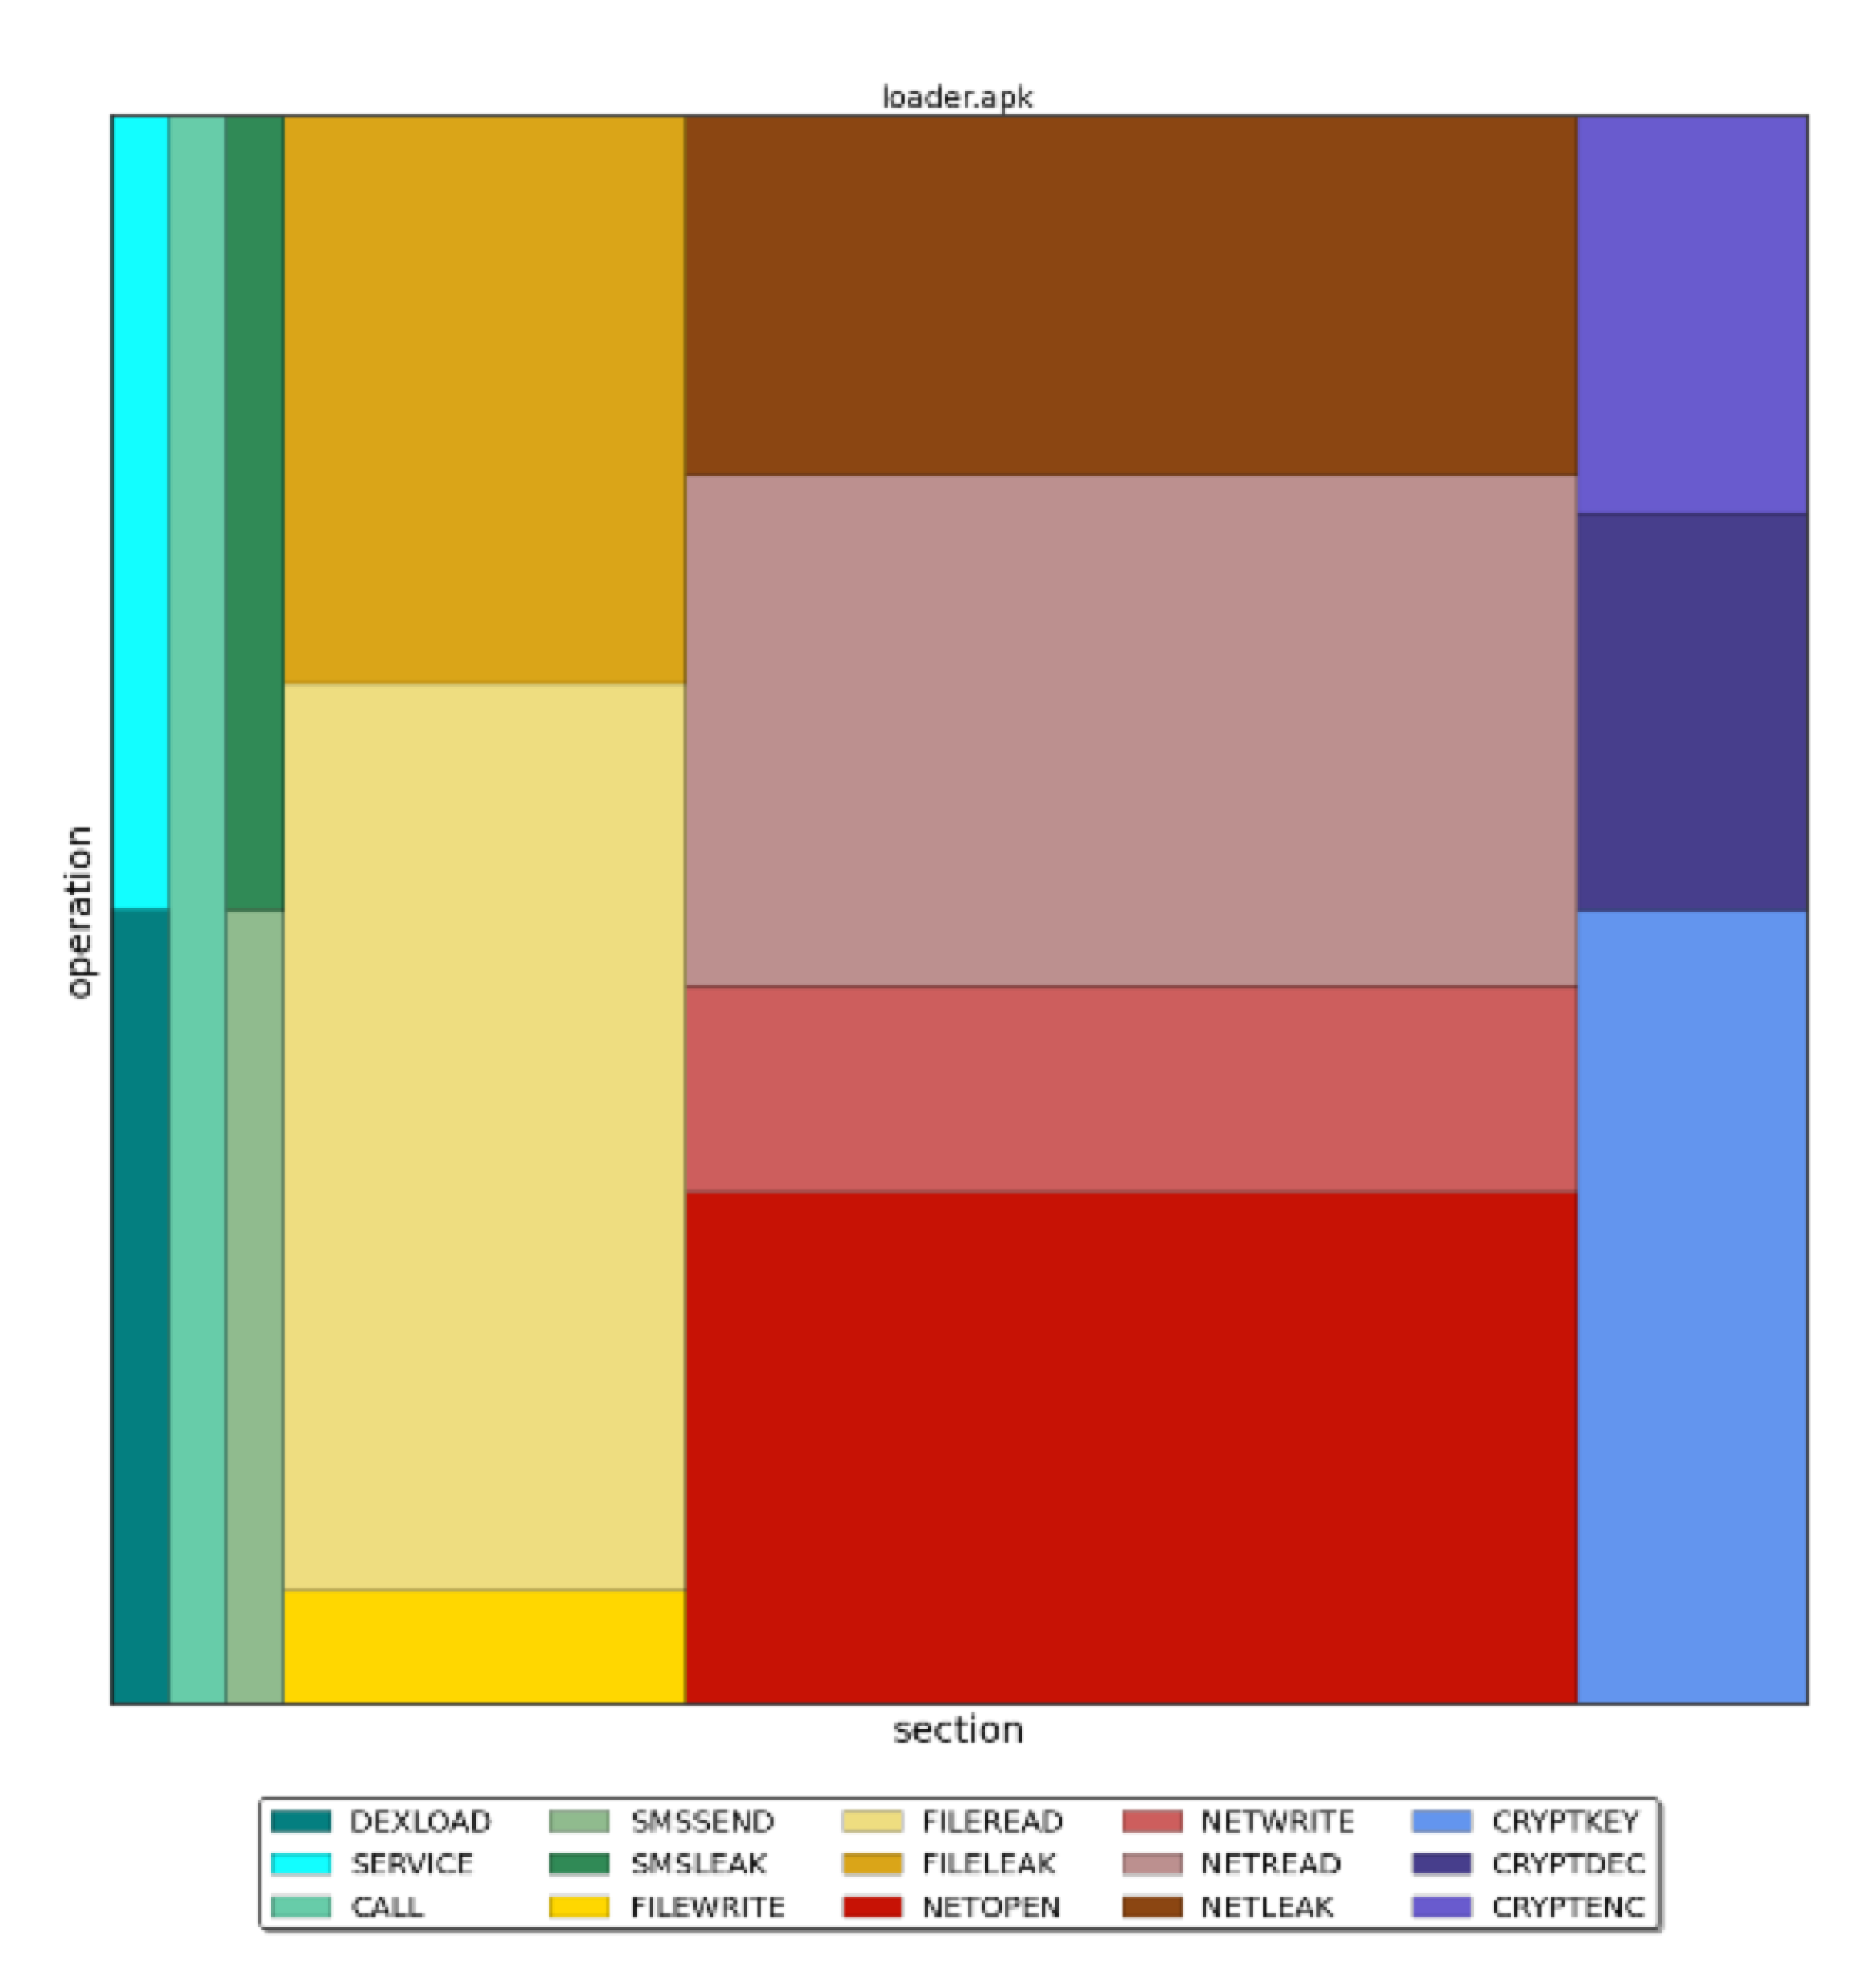
\includegraphics[scale=0.2]{droidbox2.eps}
	\end{center}
	\end{minipage}
\caption{droidbox  が生成するグラフ}
\label{droidboxgraph}
\end{figure}
\fi

\subsection{Android マルウェアを解析,調査した研究}
\label{researches}
Y.Zhou, X.Jiang は,2010 年の 8 月から 2011 年の10 月にかけて,公式サイト,非公式サイトから収集した 1,260 個,49 種類のAndroid マルウェアを用いて時系列調査と分類調査を行っている \cite{dissect} .時系列調査では,この研究で収集しているマルウェアの数 (dataset) をグラフで示している.図\ref{dataset} は その dataset の推移を表すグラフである.DroidKungFu が登場した 2011 年 6 月,AnserverBot が登場した 2011 年 10 月にこの dataset の数が急激に増えた.つまり,この 2 つのマルウェアが大きな影響を及ぼしていることがわかる.分類調査では,マルウェアのインストールの方法,起動トリガー,挙動,マルウェアが要求する権限を調査している.49 種類中,25 種類のマルウェアが Repackage によりインストールされていた.マルウェアの起動トリガーとして最も多かったのは,OS の起動時で,29 種類だった.マルウェアの挙動は,Financial charge が最も多く,その中でも,SMS を使っているものが多かった.また,多くのマルウェアが SMS, Wi-Fi に関する権限を要求していた.また,先に出てきた,2 つのマルウェアがどのような挙動をするかを示している.DroidKungFu は6 種類のヴァージョンが見つかっており,外部サーバのアドレスの格納方法が暗号化によって複雑化している.そのため,全く意味の無い文字列でも暗号化されている可能性があるのでこれらを復号して確認する必要が出てくる.よって,解析により手間がかかり,さらに難しくなってしまう.AnserverBot は解析回避と遠隔操作の2 つの特徴を持つ.AnserverBot は解析回避のために 2 つの方法をとっている.一つは自身が解析されているかどうかを検知する方法で,もう一つはメソッド名やクラス名を意図的に変えることで解析を行いにくくする方法である.

さらに,彼らは既存の 4つのセキュリティソフトがこの  dataset を検知するかどうかの調査も行った.その結果,最高は Lookout の 79.6 \% , 最低は Norton の 20.2 \% で,どのソフトウェアも検知できないマルウェアも存在した.この結果より,この 4 つのセキュリティソフトはまだ不十分であることがわかる.これらの調査結果からこの研究の結論として,マルウェアのインストール方法の中でも,最も頻繁に行われている Repackage を検知することとアプリの外部のコードの動的ローディングを防ぐ技術が必要であると彼らは主張している.この研究は Android マルウェアを調査,分類し,さらに 2 つのマルウェアについて詳しく挙動を示している.この研究では,解析手段(静的か動的か)までは言及していない.本研究では調査,分類を行うために必要となるさまざまな種類のマルウェアの挙動を正確に解析する手法を提案する.


S.Poeplau らは,マルウェアの動的に外部コードの動的ローディングに焦点をおいて解析を行っている \cite{dynamicloading} . \ref{sec:malware} で述べたように,外部コードのローディングをすることで公式ストアの検知システムをくぐり抜けることができる.また,外部コードのローディングは必ずしも不正なものではなく,マルウェア以外のアプリでも使われている.しかし,Android OS はロードされたコードをチェックしないので攻撃者はロードするものを置き換えることができる.そのためこれは Android アプリの脆弱性といえる.そこで,この研究で彼らは外部コードの動的ローディングを検知するツールを提案している.このツールは APK ファイルから取り出した DEX コードを静的に解析する.100 万回以上インストールされた,1,632 個のアプリをランダムに選び,このツールを用いて検査した.その結果,その中の 9.25 \% から外部コードのローディングの脆弱性が検知された.さらに,Google Play  での人気 50 位以内の無料アプリを同じツールで検査すると,16 \% ものアプリがその脆弱性を示した.また,彼らはこの攻撃手法に対する防御策も提案している.Dalvik VM が外部からダウンロードされたコードのハッシュ値を計算し,それが Whitelist に載っていなければ,それを実行できないようにアプリケーションに制限をかける.そうすることで,これを利用した攻撃を防ぐことができる.
外部コードの動的ローディングの応用例として,文字列としてクラス名,メソッド名を受け取り,Java の reflection を通して実行することが考えられる.reflection  とは,プログラムの実行時においてプログラム自身の構造を読み取ったり書き換えたりする技術のことである.彼らの研究では外部コードの動的ローディングの攻撃を防ぐツールを提案したが,reflection を使うと,このツールでは検知することができない.
この研究では静的解析を行っているために,外部コードのローディングは検知するが,外部コードの挙動が悪意あるものかどうかは解析しない.上記でも述べたように,外部コードのローディングは必ずしも悪意あるものとは限らない.それに対して本研究では,動的解析を行っているためにこのような外部コードの動的ローディングによる悪意ある挙動を解析することができる.


L.Yan, H.Yin はマルウェアの動的解析環境 (DroidScope) を提案している \cite{droidscope} .彼らは Android SDK が提供するエミュレータをベースに自分たちで手を加えて,そのエミュレータの中でマルウェアを動かしている.彼らは Android システム全体の再構築を行っている.つまり,DroidScope はハードウェア,Linux OS (Android は Linux をベースにして動作している),Dalvik VM の 3 種類の API を提供する.DroidScope が提供する API を用いることで,Android API, Dalvik VM, Linux , さらには機械語の命令までをトレースするツールを提案している.{\it API tracer, native tracer, Dalvik instruction tracer} の 3 つである.また,これらの API に動的な taint analysis を実行することで,情報漏えいを解析するツール ({\it Taint tracker}) も提案している.彼らはこの 4 つのツールのパフォーマンス測定も行っている.元のエミュレータで実行時間を基準に,4 つのツールの実行時間を調べた.その結果,オーバーヘッドは小さいと言える結果であった.しかし,taint traker は他の 3 つのツールとくらべて大きなオーバーヘッドを示した.彼らはこれらのツールを用いて先に述べた,DroidKungFu を解析した.この解析によって,このマルウェアのルート権限を取得する方法と情報を盗み出す方法を明らかにしている.DroidKungFu だけでなく,論文中では DroidDream も解析している.DroidKungFu の場合と同様な解析を行った結果,DroidDream が端末識別番号を盗み出す方法を突き止めた.DroidScope は 1 つの実行パスのみを解析しない.彼らは実行パスを増やすために,システムコール,ネイティブ API,Dalvik メソッドなどの返り値を変えることで,異なる実行パスを実現した. symbolic execution のほうが,より良いことが考えられるが,かれらはこれを今後の課題としている.彼らの研究は実行された API,メソッドを動的に得ることで解析を行っているため,解析のためのアプローチは本研究と共通している点がある.しかし,本研究は実機で行っているのに対して,彼らの研究はエミュレータ上で行っている.もし,マルウェアがエミュレータ上で動作しているのを検知して,振る舞いを変える可能性もある.デスクトップ PC を標的にしたマルウェアは実際に振るまいを変えることがわかっている \cite{detection} \cite{emulation} \cite{v2e} . DroidScope のような解析ツールが普及するにつれて,エミュレータでの実行を検知するマルウェアが出てくるだろうと,彼らはこの論文中で述べている.本研究が提案している実機による解析であればマルウェアの "正常" な動作を解析することができる.

マルウェアを解析している方法としては,動的解析と静的解析がある.S.Poelau らは外部コードの動的ローディングを用いるマルウェアを静的解析により検知する手法を提案している.しかし,静的解析であるために,実際に外部からコードを受け取ってその結果実行されるマルウェアの挙動を解析することはできない.L.Yan, H.Yin が提案する DroidScope はエミュレータ上で動的にマルウェアを解析している.エミュレータで実行する場合と実機で実行する場合では,厳密に同じ環境であるとはいえない.エミュレータでの解析を検知する機能を持ったマルウェアが将来出てきた場合,DroidScope はマルウェアを解析することができなくなってしまう.そこで,本研究では実機でマルウェアを実行して解析を行う.

\begin{figure}[t]
\begin{center}
\graphicspath{{./epsfiles/}}
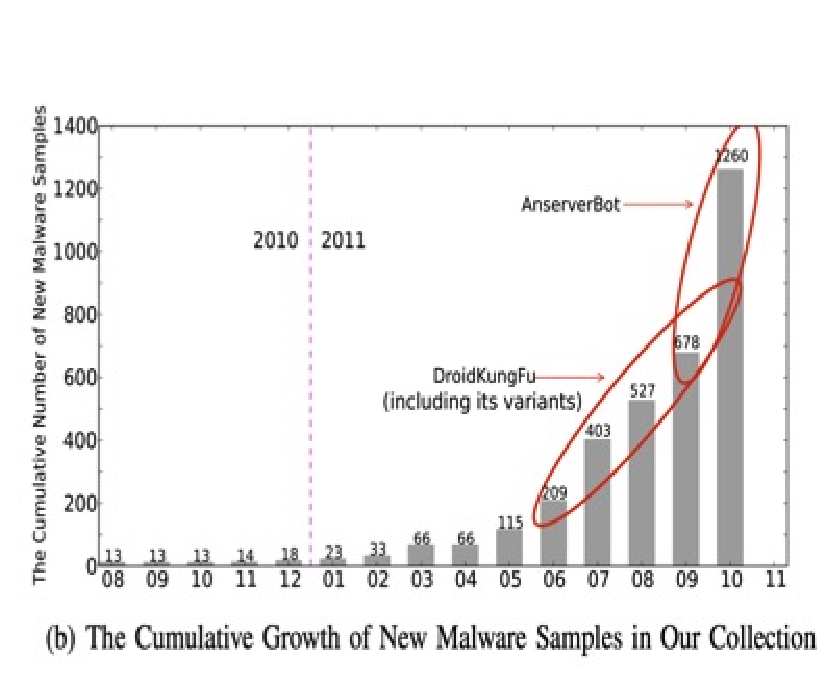
\includegraphics[ scale = 0.5]{graph.eps}
\end{center}
\caption{マルウェアの dataset の推移}
\label{dataset}
\end{figure}
